\chapter{Tinjauan Pustaka dan Dasar Teori}

\section{Tinjauan Pustaka}

\subsection{Apakah Pola Deteksi Duplikat (CDP) dapat Disalin}
CDP dinilai dapat digunakan untuk mendeteksi pemalsuan, sehingga akhir-akhir ini mendapatkan banyak perhatian dari akademisi dan industri. Tingkat keamanan CDP
dalam mendeteksi serangan pemalsuan yang canggih telah dipelajari secara teoritis dan praktis dalam beberapa penelitian, namun hasilnya masih belum sepenuhnya
meyakinkan \cite{PICARDCANCOPYDETECTIONPATTERN}. Kontribusi utama dari penelitian ini adalah untuk menyajikan \emph{dataset} secara publik dan berbagai jenis
contoh penyerangan terdapat CDP tersebut, sehingga kinerja CDP terhadap beberapa penyerangan dapat diketahui. \emph{Dataset} CDP tersebut terdiri dari lebih
dari 27.500 gambar CDP dan merupakan \emph{dataset} CDP terbesar hingga saat ini \cite{PICARDCANCOPYDETECTIONPATTERN}. Kontribusi selanjutnya adalah meneliti
tentang kinerja detektor CDP dalam mendeteksi CDP orisinal ataupun salinan. Verifikasi dari CDP dapat dilakukan dengan perangkat seluler, tanpa harus
menggunakan pemindai khusus \cite{WONG2017}, \cite{SCHRAML2018REAL}. Dengan \emph{dataset} dan detektor yang dibuat, peneliti sebelumnya ingin menguji
validitas hipotesis bahwa CDP yang dicetak berulang kali akan terdegradasi kualitasnya dan dapat dideteksi sebagai CDP palsu
\cite{PICARDCANCOPYDETECTIONPATTERN}. Kontibusi terakhir dari penelitian ini adalah meneliti beberapa metode yang dapat dilakukan untuk meningkatkan performa
klasifikasi dari model.

\begin{figure}[!ht]
	\centering
	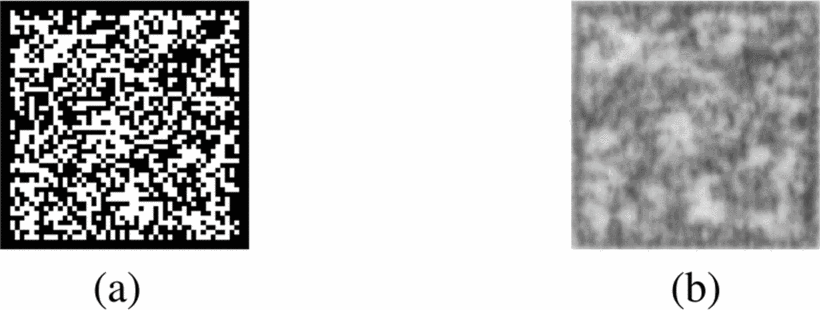
\includegraphics[width=12cm]{contents/chapter-2/2-cdporivsfake.png}
	\caption[Contoh dari CDP a) CDP \emph{template} digital ($I$) b) CDP yang telah terdegradasi kualitasnya akibat proses P\&S ($\widetilde{I}$)]{Contoh dari CDP a) CDP \emph{template} digital ($I$) b) CDP yang telah terdegradasi kualitasnya akibat proses P\&S ($\widetilde{I}$) \cite{PICARDCANCOPYDETECTIONPATTERN}}
	\label{Fig: 2-cdporivsfake}
\end{figure}

\subsubsection{Prinsip Degradasi Informasi}
Prinsip dari pendeteksian CDP palsu dilakukan berdasarkan hilangnya informasi, yang mana muncul dari proses P\&S \cite{picard2004digital}. Proses P\&S
merupakan proses stokastik (mempunyai unsur peluang atau kebolehjadian) \cite{phan2014document}, yang menyebabkan perubahan struktur dan kualitas gambar pada
CDP, seperti yang ditampilkan pada Gambar \ref{Fig: 2-cdporivsfake} derau yang dihasilkan dari proses P\&S CDP sulit untuk dikarakterisasi
\cite{picard2008security} karena setiap \emph{printer} dan pemindai memiliki karakteristiknya sendiri.

\begin{figure}[!ht]
	\centering
	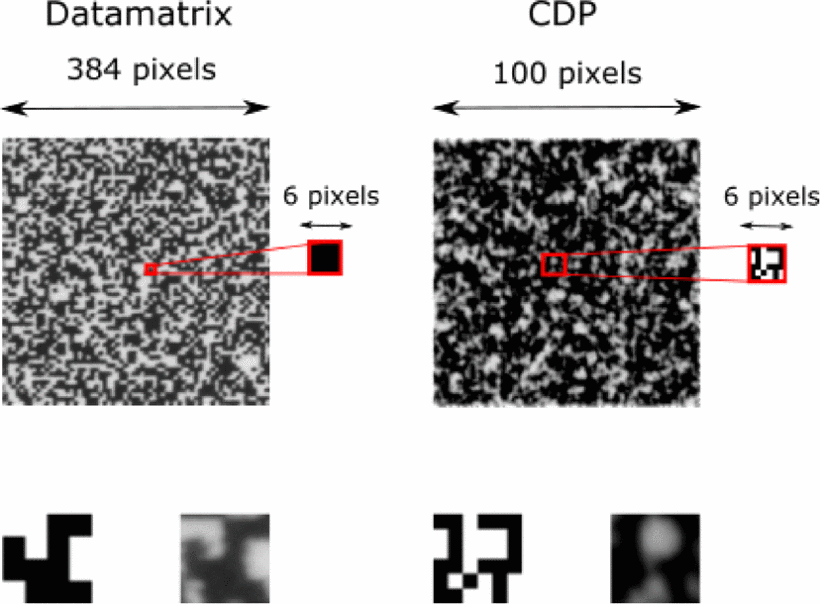
\includegraphics[width=10cm]{contents/chapter-2/2-datamatrixvscdp.png}
	\caption[Perbandingan dari CDP dengan data-matriks: Data-matriks memiliki ukuran unit komponen yang lebih besar, sehingga degradasi informasi tidak berdampak signifikan pada struktur kode]{Perbandingan dari CDP dengan data-matriks: Data-matriks memiliki ukuran unit komponen yang lebih besar, sehingga degradasi informasi tidak berdampak signifikan pada struktur kode \cite{PICARDCANCOPYDETECTIONPATTERN}}
	\label{Fig: 2-datamatrixvscdp}
\end{figure}

CDP sering dibandingkan dengan kode batang dua dimensi seperti data-matriks karena kemiripan visualnya. Namun, seperti yang diilustrasikan pada Gambar
\ref{Fig: 2-datamatrixvscdp}, unit elemen data-matriks jauh lebih besar dibandingkan unit elemen CDP. Oleh karena itu, prinsip kehilangan atau degradasi
informasi tidak berdampak pada struktur data-matriks. Sebagai contoh, korelasi antara data-matriks \emph{template} digital hasil \emph{generate} dengan versi
rusak akibat proses P\&S bisa lebih dari 0,9, sedangkan korelasi antara CDP \emph{template} digital hasil \emph{generate} dengan versi rusak akibat proses
P\&S-nya hanya sekitar 0,45 s.d. 0,55 tergantung pada perangkat pemindai dan pencetaknya. Oleh karena itu, ukuran dari unit elemen pola CDP, yaitu 100 x 100
piksel seperti yang ditampilkan pada Gambar \ref{Fig: 2-datamatrixvscdp}, ukuran pola keseluruhan juga sangat mempengaruhi proses autentikasi dan kemampuan
pemalsu dalam mereproduksi pola. Pada praktiknya, ukuran unit elemen pada CDP adalah 1 x 1 piksel atau 2 x 2 piksel agar bisa memanfaatkan prinsip degradasi
informasi secara maksimal.

\subsubsection{Definisi Teoritis dari Sistem Autentikasi CDP}
Autentikasi dari CDP terdiri dari dua langkah utama. Langkah pertama adalah langkah registrasi di mana pola dihasilkan kemudian dicetak dengan pencetak untuk
menghasilkan CDP orisinal. Langkah kedua adalah verifikasi CDP, menggunakan sebuah perangkat pemindai yang telah terautentikasi (perangkat seluler dengan
kamera), CDP dipindai dan dilewatkan melalui tes autentikasi (dengan parameter-parameter pemindaian tertentu). Jika tes tersebut positif, item dianggap
autentik.

Upaya penyerangan yang paling sering dilakukan oleh pembajak adalah sebagai berikut: Pembajak melakukan pemindaian CDP pada sebuah item menggunakan pemindai
beresolusi tinggi, mengestimasi pola asli dari CDP, kemudian mencetak pola yang telah diestimasi menggunakan pencetak beresolusi tinggi. Pada skenario ini $I$
merupakan CDP \emph{template} digital hasil \emph{generate}, kemudian $\Pi(I)$ merupakan CDP \emph{template} digital yang dicetak, dengan $\Pi(\cdot)$
\emph{noise} yang dihasilkan dalam proses pencetakan menggunakan pencetak yang telah terautentikasi. Selanjutnya, proses autentikasi dapat dirumuskan sebagai
uji hipotesis berikut ini:

\begin{align}
	 & \mathcal{H}_{0}:\tilde{I}\sim\Sigma(\Pi(I)), \\ &\mathcal{H}_{1}:\tilde{I}\not\sim\Sigma(\Pi(I)),\nonumber
\end{align}

\noindent di mana $\widetilde{I}$ adalah gambar CDP \emph{grayscale} yang diterima oleh pusat autentikasi. $\widetilde{I}$ dapat berupa CDP orisinal (i.e. $\Sigma(\Pi(I))$) atau CDP palsu (i.e. $\Sigma(\Pi'(\hat{I}))$). Metriks yang digunakan untuk membandingkan CDP orisinal dengan palsu adalah koefisien jarak ataupun korelasi \cite{dirik2012copy}.

\subsubsection{Komponen dari Detektor}
Hasil menunjukkan bahwa autentikasi menggunakan CDP \emph{raw grayscale} lebih efisien dibandingkan dengan CDP yang telah di-\emph{thresholding}
\cite{phan2014document}. Kemudian, secara umum, ada beberapa langkah yang dilakukan untuk melakukan autentikasi CDP, antara lain:

\begin{itemize}
	\item Melakukan \emph{resizing} pada \emph{template} CDP menggunakan faktor skala tertentu.
	\item Menggunakan teknik pencocokan \emph{template} dengan mengambil sub-bagian dari CDP.
	\item Menggunakan \emph{high pass filtering} (seperti \emph{unsharp masking}) sebelum melakukan penyekoran korelasi.
\end{itemize}

\subsection{Deteksi Pembajakan menggunakan SQR}
Pendekatan keamanan tradisional pada produk sebelumnya sudah diimplementasikan melalui \emph{taggant}, hologram, dan tinta keamanan. Beberapa metode tersebut
memang mudah diimplementasikan, mudah diverifikasi, dan murah. Namun, dalam sebuah kode QR metode-metode tersebut belum dapat diimplementasikan. Produk yang
ditempeli oleh kode QR palsu biasanya masih dapat dipindai dan mengembalikan keluaran sama dengan produk orisinal. Penelitian yang dilakukan oleh Justin
Picard, Paul Landry, dan Michael Bolay ini membahas tentang bagaimana mengimplementasikan CDP ke dalam SQR untuk mendeteksi kode QR palsu
\cite{picard2021counterfeit}.

\begin{figure}[!ht]
	\centering
	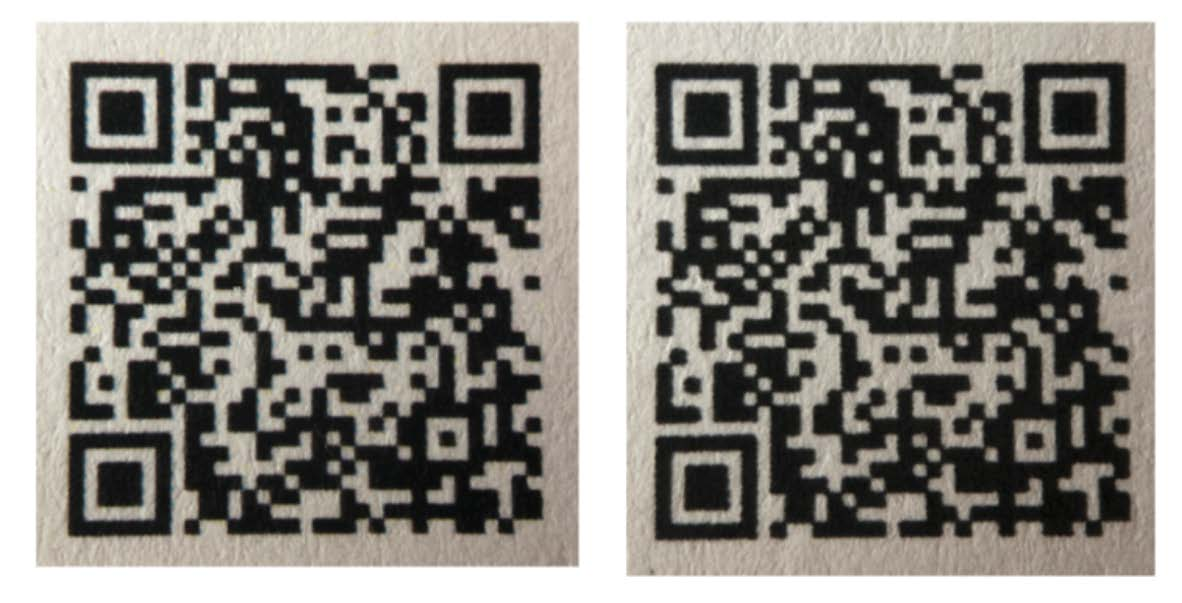
\includegraphics[width=10cm]{contents/chapter-2/2-qrorivspalsu.jpg}
	\caption[Perbandingan dari kode QR orisinal dan palsu, keduanya menyimpan informasi yang sama dan sama-sama dapat dipindai]{Perbandingan dari kode QR orisinal dan palsu, keduanya menyimpan informasi yang sama dan sama-sama dapat dipindai \cite{picard2021counterfeit}}
	\label{Fig: 2-qrorivspalsu}
\end{figure}

Pada Gambar \ref{Fig: 2-qrorivspalsu} terlihat bahwa sangat sulit untuk membedakan antara kode QR orisinal dan palsu hasil replikanya, apalagi jika tidak ada
pembandingnya. Skenario yang dapat dilakukan oleh pembajak dalam menerbitkan kode QR palsu dapat dilihat pada Gambar \ref{Fig: 2-counterveiterpractice}. Kode
QR palsu dipindai dengan perangkat beresolusi tinggi, kemudian dicetak ulang. Harapannya dengan CDP yang diletakkan pada kode QR, kode QR palsu yang dipindai
untuk autentikasi dapat terdeteksi sebagai kode QR palsu, lihat pada Gambar \ref{Fig: 2-counterveiterpractice}.

\begin{figure}[!ht]
	\centering
	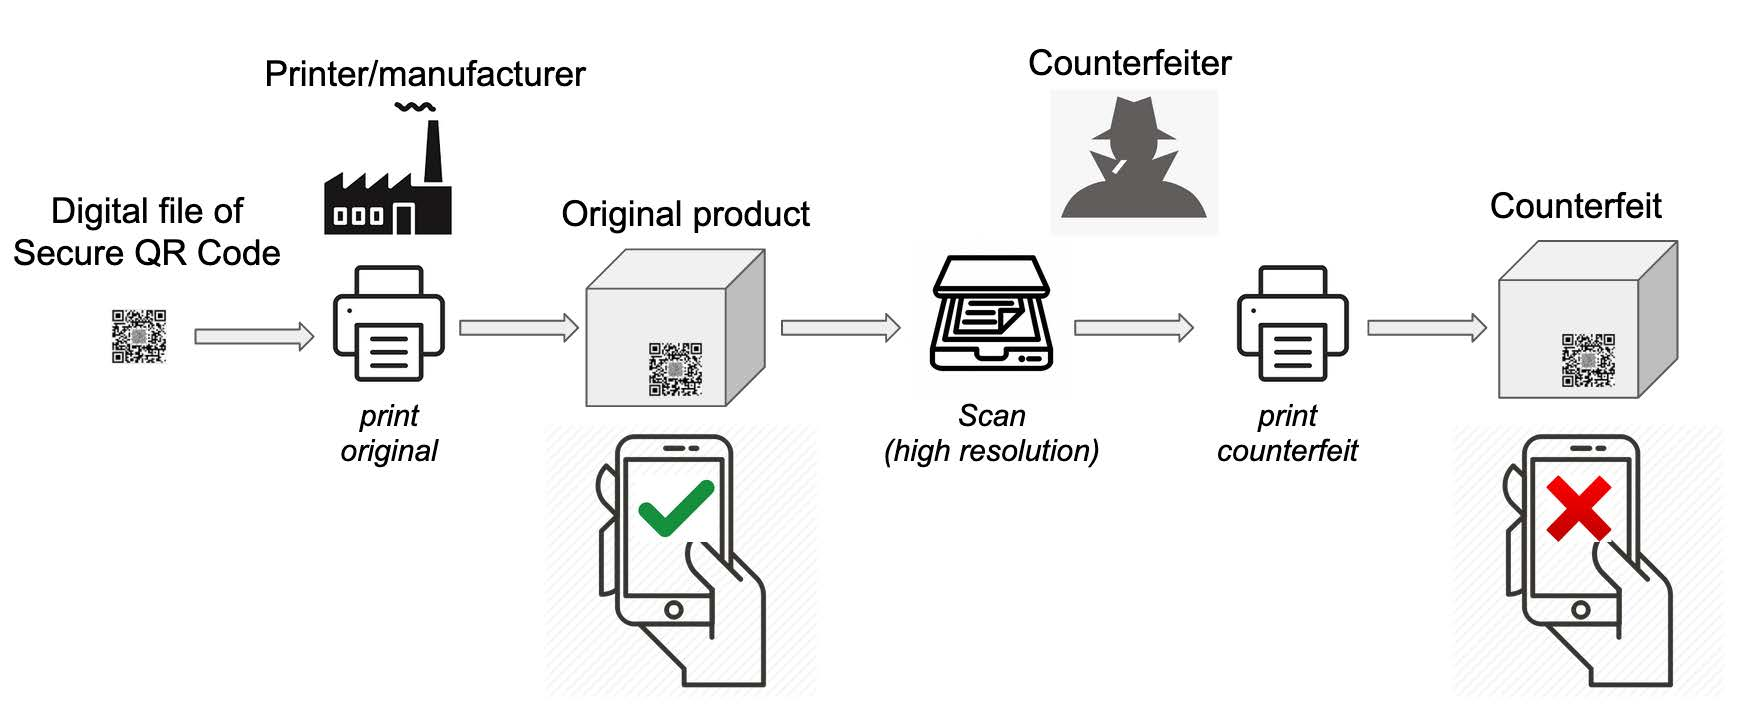
\includegraphics[width=12cm]{contents/chapter-2/2-counterveiterpractice.jpg}
	\caption[SQR diharapkan dapat mendeteksi kode QR palsu pada saat diautentikasi oleh pengguna]{SQR diharapkan dapat mendeteksi kode QR palsu pada saat diautentikasi oleh pengguna \cite{picard2021counterfeit}}
	\label{Fig: 2-counterveiterpractice}
\end{figure}

\subsubsection{Struktur dari SQR}
\begin{figure}[h]
	\centering
	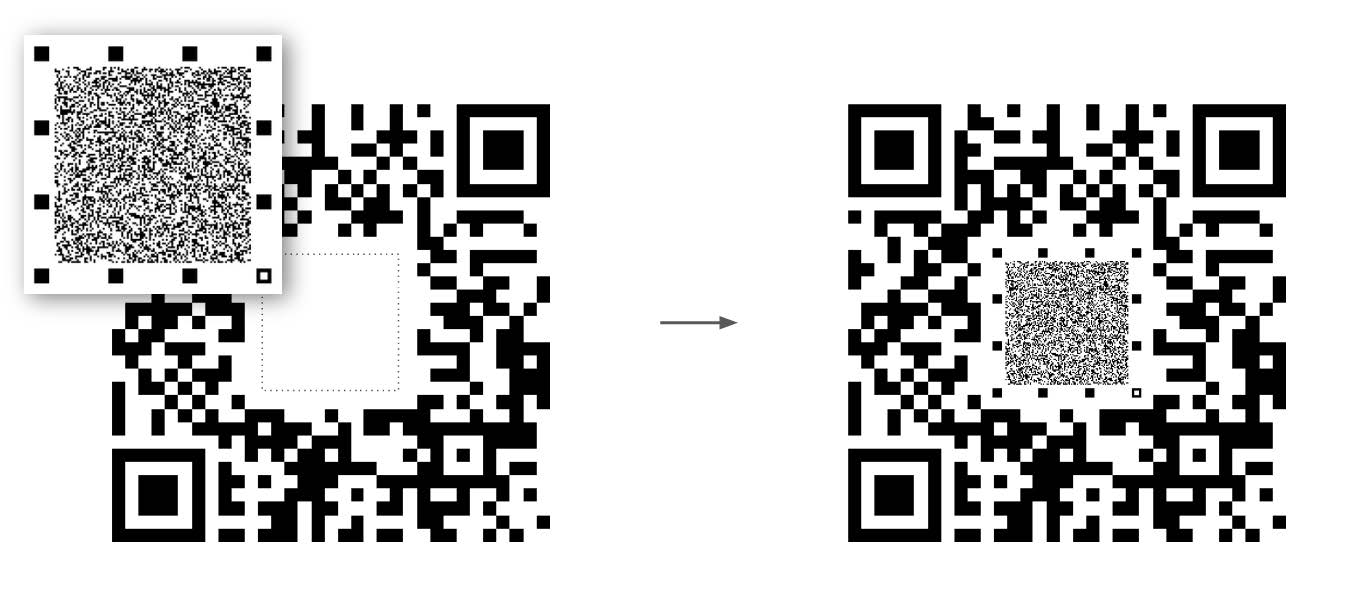
\includegraphics[width=12cm]{contents/chapter-2/2-struktursqr.jpg}
	\caption[Struktur SQR secara umum]{Struktur SQR secara umum \cite{picard2021counterfeit}}
	\label{Fig: 2-struktursqr}
\end{figure}

Secara umum, CDP akan diletakkan di tengah-tengah dari kode QR. CDP nantinya akan digunakan untuk proses autentikasi. Di sekitar CDP diletakkan beberapa
penanda untuk memudahkan program dalam mendeteksi dan mendapatkan objek CDP (lokalisasi CDP). CDP mungkin ditempelkan di tengah-tengah kode QR karena adanya
fitur koreksi kesalahan dalam kode QR. Ada empat jenis koreksi kesalahan pada kode QR: L, M, Q, dan H, yang secara teoritis memiliki kemampuan untuk memulihkan
informasi yang hilang sebesar 7\%, 15\%, 25\%, dan 30\% kerusakan pada kode QR. Pada penelitian ini, area yang dirusak untuk meletakkan CDP adalah sebesar 1/9
dari ukuran awal kode QR. Aplikasi yang digunakan untuk melakukan autentikasi pada perangkat pemindai (perangkat seluluer) hanya mengambil objek CDP saja, hal
tersebut memiliki beberapa keuntungan, area yang digunakan untuk autentikasi menjadi lebih spesifik, sehingga kecepatan deteksi akan lebih cepat, fokus dari
kamera juga relatif akan lebih baik karena mengambil objek yang lebih kecil dan terfokus, selain itu karena sistem autentikasi berada di \emph{remote server}
yang mana data akan dikirim dari perangkat seluler pemindai, semakin kecil area yang dikirimkan, semakin hemat \emph{bandwith} yang digunakan.

\subsubsection{Pembuatan dan Pencetakan SQR}
CDP yang digunakan dalam penelitian ini menggunakan dua level \emph{grayscale} atau biner. Resolusi mesin \emph{printer} yang digunakan adalah 812,8 ppi dengan
merek HP Indigo. CDP di-\emph{generate} menggunakan \emph{pseudo-random number generator}, menggunakan \emph{seed} tertentu. CDP dapat dibuat unik untuk setiap
kode QR ataupun sama pada sekelompok kode QR tertentu. Dalam melakukan pencetakan dan pemindaian SQR, perangkat pencetak dan pemindai akan diverifikasi
terlebih dahulu dengan konfigurasi dan parameter tertentu untuk menjamin kualitas dari pencetakan.

\subsubsection{Autentikasi SQR}
Perangkat pemindai QR biasa sudah pasti dapat melakukan \emph{decode} informasi dari kode QR, namun untuk melakukan autentikasi terhadap CDP, tentunya
diperlukan aplikasi khusus. Aplikasi khusus ini berjalan di perangkat seluler, secara umum proses pemindaian yang dilakukan oleh aplikasi khusus tersebut
adalah sebagai berikut:

\begin{itemize}
	\item Aplikasi akan melakukan pemindaian per-\emph{frame} dari kamera hingga mendapatkan kode QR.
	\item Kode QR akan di-\emph{decode} untuk mengekstrak informasi dalam kode QR.
	\item Indeks kualitas pemindaian akan dikalkulasi berdasarkan \emph{frame} yang didapatkan.
	\item Jika indeks kualitas pemindaian dinilai cukup tinggi, area CDP akan dideteksi, dipotong, dan dikirim ke \emph{remote server} bersamaan dengan informasi dari
	      kode QR yang telah ter-\emph{decode} untuk autentikasi.
\end{itemize}

\begin{figure}[!ht]
	\centering
	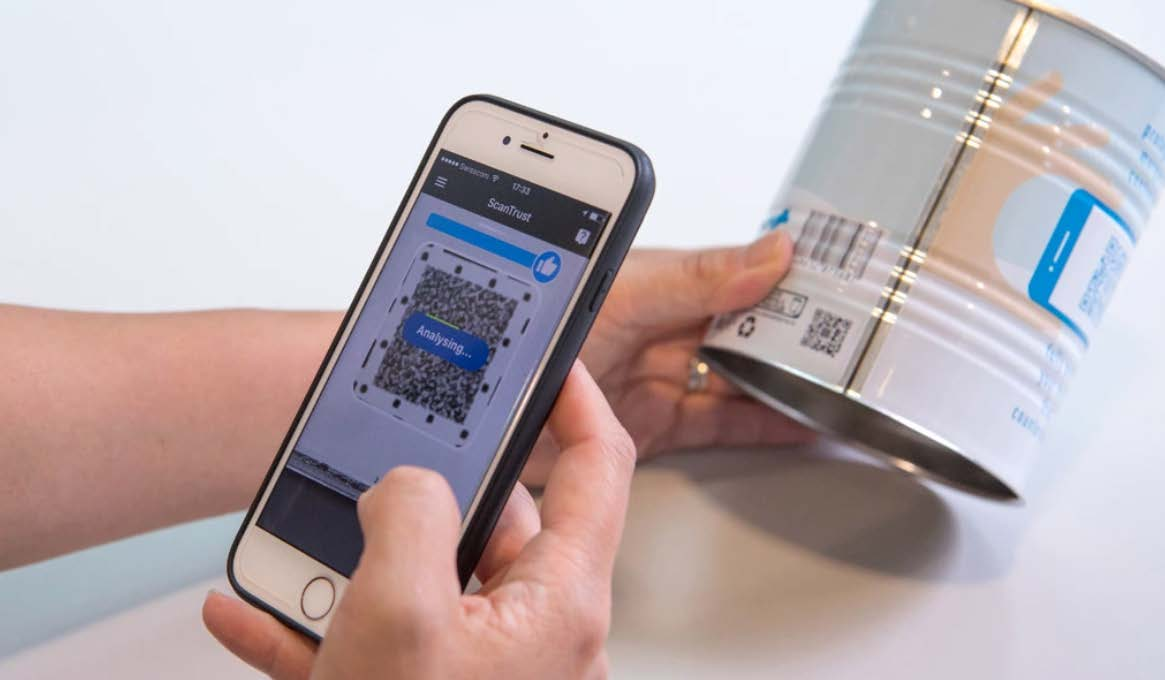
\includegraphics[width=11cm]{contents/chapter-2/2-pemindaiansqr.jpg}
	\caption[Perangkat seluler melakukan pemindaian menggunakan aplikasi khusus]{Perangkat seluler melakukan pemindaian menggunakan aplikasi khusus \cite{picard2021counterfeit}}
	\label{Fig: 2-pemindaisqr}
\end{figure}

\noindent Setelah \emph{server} mendapatkan CDP yang telah dipotong beserta informasi data kode QR, autentikasi yang dilakukan di \emph{server} adalah sebagai berikut:

\begin{itemize}
	\item \emph{Identifier} unik akan diekstrak dari informasi kode QR yang didapatkan yang mana dibutuhkan sebagai parameter autentikasi.
	\item \emph{Template} CDP digital akan di-\emph{generate}.
	\item Matriks similaritas akan dikalkulasi dari perbandingan antara CDP yang dikirimkan dari hasil pemindaian dengan CDP \emph{template} yang di-\emph{generate}.
	\item Penyesuaian lain seperti, ketajaman gambar, filter akan dilakukan untuk memperoleh hasil terbaik.
	\item Normalisasi nilai fitur akan dilakukan.
	\item Keluaran berupa CDP "orisinal", "palsu", atau "pemindaian buruk" akan dikeluarkan oleh \emph{server} (pemindaian buruk bisa disebabkan oleh hasil gambar yang
	      kabur).
\end{itemize}

\subsection{Autentikasi Digital menggunakan CDP}
Penelitian ini memberikan solusi atas permasalahan pembajakan produk dengan membuat sebuah gambar digital dengan properti tertentu, yang disebut dengan
\emph{Copy detection patterns} (CDP), yang akan diletakkan pada produk ataupun dokumen. Penelitian ini merupakan salah satu penelitian awal dari
penelitian-penelitian selanjutnya tentang pengembangan CDP untuk deteksi pembajakan. Permasalahan yang coba dibahas pada penelitian ini adalah apakah mungkin
untuk membuat dokumen salinan yang sempurna? Untuk menjawab pertanyaan tersebut peneliti melakukan eksperimen untuk mendemonstrasikan kelayakan penerapan CDP
untuk mengamankan dokumen dari pemalsuan \cite{picard2004digital}.

\noindent Spesifikasi CDP dan perangkat yang digunakan dalam penelitian adalah sebagai berikut:
\begin{itemize}
	\item Gambar CDP berukuran 100x100 piksel, dicetak dengan ukuran 0,72cm$^2$.
	\item \emph{Printer}: \emph{Printer} laser kantor standar dengan 1200 dpi.
	\item \emph{Pemindai}: Canon 1240 pada 300 dpi \emph{grayscale} dan 200 dpi \emph{grayscale}.
\end{itemize}

\noindent Kemudian, ada tiga jenis data kopian yang diproduksi, yaitu:
\begin{itemize}
	\item Salinan pemindai: Dibuat menggunakan Epson 1650 pada 2400 dpi dan dicetak ulang dengan \emph{printer} dan kertas yang sama dengan CDP orisinal.
	\item Fotokopi berwarna
	\item Pola yang dibuat ulang
\end{itemize}

\noindent Hasil dari percobaan tersebut adalah:
\begin{itemize}
	\item Indeks kualitas maksimum 100 hanya diperoleh dengan CDP digital. Proses P\&S menyebabkan penurunan kualitas, pembuatan salinan dari cetakan pertama juga
	      menyebabkan penurunan kualitas lagi.
	\item Resolusi pemindaian yang lebih rendah memengaruhi hasil secara signifikan pada cetakan orisinal dibandingkan pada cetakan salinan. Namun, perbedaan antara
	      dokumen asli dan salinan tetap dapat dibedakan secara signifikan.
	\item Salinan yang dibuat ulang dengan mengestimasi pola memiliki indeks kualitas mendekati nol, hal tersebut disebabkan nilai pikselnya hampir tidak berkorelasi
	      sama sekali dengan \emph{template} digital.
	\item Salinan berkualitas lebih baik dapat dibuat dengan mencetak ulang hasil pindaian beresolusi tinggi pada kertas yang memiliki noda tinta lebih sedikit (misal
	      kertas foto) dan dengan \emph{printer} yang lebih baik. Namun, membuat salinan seperti itu akan sangat menambah beban pemalsu. Selain itu, hasil salinannya
	      akan terlihat berbeda dengan mata telanjang dan tetap memiliki indeks kualitas yang jauh lebih rendah daripada aslinya.
\end{itemize}

\noindent Kesimpulan yang didapatkan dari penelitian ini \cite{picard2004digital} antara lain:
\begin{itemize}
	\item Setiap kali gambar dicetak dan dipindai (proses P\&S), kualitasnya akan menurun dan terdegradasi. Hal ini disebabkan oleh sifat dari \emph{printer}, kertas,
	      dan pemindai.
	\item Sebagian besar gambar jenis dokumen belum menerapkan prinsip degradasi informasi untuk melindungi produk dari pembajakan.
	\item Berlawanan dengan gambar dokumen, gambar yang terdiri dari derau murni dapat terdegradasi secara maksimal, sehingga akan mudah membedakan gambar orisinal dan
	      palsunya.
	\item CDP adalah gambar dengan entropi maksimum yang dihasilkan dengan menggunakan sebuah kunci rahasia. CDP umumnya disisipkan pada gambar digital yang akan dicetak
	      atau langsung dicetak pada dokumen.
	\item CDP tidak cocok untuk dideteksi dengan mata telanjang, namun akan sangat efektif dideteksi menggunakan komputer.
\end{itemize}

\section{Dasar Teori}

\subsection{Kode QR}

Kode QR (\emph{Quick Response}) adalah sebuah kode matriks dua dimensi (2-D) yang dapat dibaca oleh komputer. Kode QR dua dimensi dapat menyimpan data yang
lebih banyak dibandingkan dengan kode satu dimensi (\emph{barcode}) dengan ruang yang lebih kecil. Selain itu, kode QR memiliki fitur koreksi kesalahan
pembacaan dan beberapa fitur unik lainnya \cite{densoqrcode}.

Seperti bahasa tertulis lainnya, kode batang atau \emph{barcode} merupakan representasi visual dari informasi. Namun, berbeda dengan bahasa yang dapat dibaca
oleh manusia, kode batang dirancang untuk dibaca dan dipahami oleh komputer atau mesin. Menggunakan sistem penglihatan dari mesin berupa pemindai laser optik
ataupun kamera dan perangkat lunak yang dapat menginterpretasikan kode batang. Aturan bagaimana \emph{barcode} dikonstruksikan disebut sebagai \emph{grammar},
sedangkan set karakter yang digunakan (alfabet) disebut \emph{symbology} \cite{densoqrcode}.

\subsubsection{Bagaiamana Kode QR Bekerja}
\begin{figure}[!ht]
	\centering
	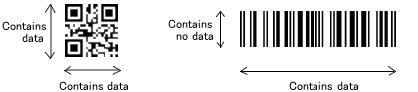
\includegraphics[width=12cm]{contents/chapter-2/2-2dvs1dcode.jpg}
	\caption[Perbandingan 1-D dengan 2-D \emph{barcode}]{Perbandingan 1-D dengan 2-D \emph{barcode} \cite{densoqrcode}}
	\label{Fig: 2-2dvs1dcode}
\end{figure}

Tidak seperti kode batang satu dimensi, kode QR adalah matriks 2-D yang menyimpan informasi dalam tiap modul di baris dan kolomnya yang memiliki gelap dan
terang tertentu.

\begin{figure}[!ht]
	\centering
	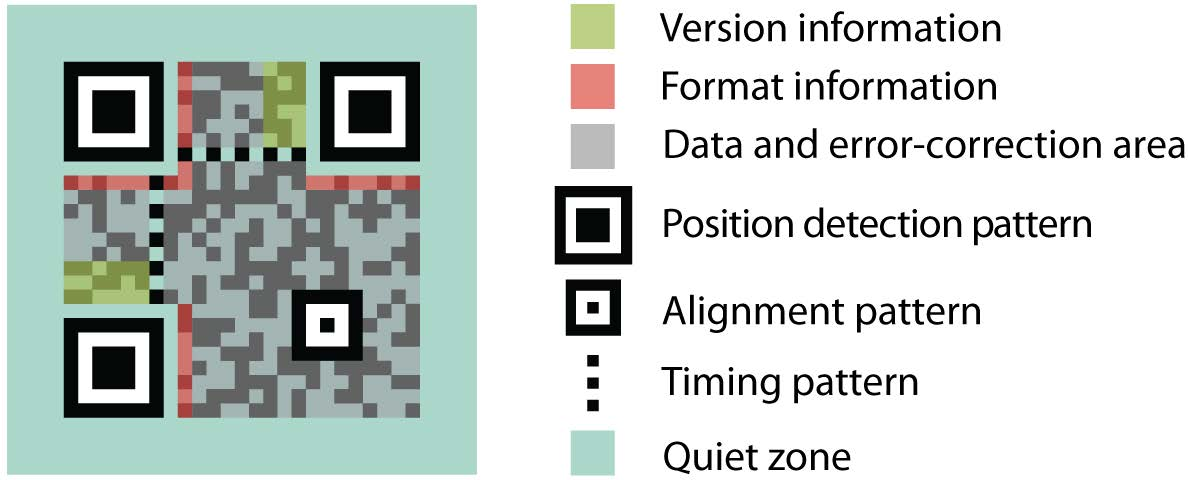
\includegraphics[width=10cm]{contents/chapter-2/2-strukturqrasli.jpg}
	\caption[Struktur modul pada kode QR dua dimensi]{Struktur modul pada kode QR dua dimensi \cite{densoqrcode}}
	\label{Fig: 2-strukturqrasli}
\end{figure}

Setiap modul dalam kode QR memiliki fungsi-fungsi tertentu. Beberapa modul berisi tentang informasi yang tersimpan dalam kode QR itu sendiri, dengan lainnya
dibagi menjadi beberapa grup berdasarkan fungsinya. Untuk memastikan kode QR dapat dipindai dari berbagai sisi, ada tiga modul \emph{position detection
	pattern} yang terletak di ketiga sudut yang memungkinkan kode QR untuk dipindai dari 360$^{\circ}$.

\subsubsection{Versi Kode QR}
Kode QR dapat di-\emph{generate} dari 40 versi yang berbeda, dari yang berukuran 21x21 modul (versi 1) hingga 177x177 modul (versi 40).

\begin{figure}[h]
	\centering
	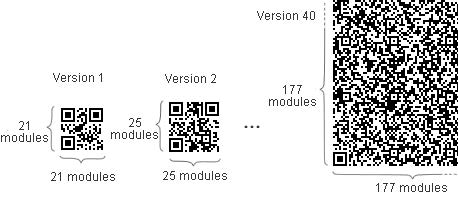
\includegraphics[width=10cm]{contents/chapter-2/2-versiqr.jpg}
	\caption{Jumlah modul berdasarkan versi kode QR}
	\label{Fig: 2-versiqr}
\end{figure}

Setiap kenaikan satu versi, maka akan ada penambahan 4 modul, sehingga dapat memuat data atau informasi yang lebih banyak. Jumlah maksimum data yang dapat
disimpan tergantung pada versi kode QR, tipe karakter, dan besar toleransi kesalahan.

\subsubsection{Koreksi Kesalahan Kode QR}
Koreksi kesalahan kode QR mengimplementasikan \emph{Reed-Solomon codes}, yang mana merupakan salah satu metode koreksi kesalahan matematis yang banyak
digunakan. Hal ini memungkinkan kode QR tetap dapat dibaca walaupun dalam kondisi kotor ataupun rusak dengan batasan tertentu. Ada empat tipe koreksi kesalahan
standar yang ada dalam kode QR. Semakin tinggi level koreksi kesalahan, semakin besar toleransi terhadap kerusakan kode QR, namun semakin besar juga versi kode
QR-nya.

\begin{table}[h]
	\caption{Tabel perbandingan level koreksi kesalahan dengan persentase toleransi kesalahannya}
	\vspace{0.5em}
	\centering
	\begin{tabular}{|c|c|c|}
		\hline
		Level Koreksi Kesalahan & Besar Toleransi Kesalahan \\
		\hline
		L                       & 7\%                       \\
		M                       & 15\%                      \\
		Q                       & 25\%                      \\
		H                       & 30\%                      \\ \hline
	\end{tabular}
	\label{Tab: 2-tabelperbandinganlevelkoreksi}
\end{table}

Dalam memilih level koreksi kesalahan, sebaiknya disesuaikan dengan kondisi lingkungan di mana kode QR tersebut digunakan. Misalnya dalam kondisi lingkungan
yang bersih, level L (7\%) dapat digunakan. Secara umum, level yang paling sering digunakan adalah level M (15\%).

\subsection{\emph{Copy Detection Pattern} (CDP)}
Pola deteksi duplikat (CDP) adalah sebuah gambar berpola dengan entropi tinggi yang dibuat menggunakan kode rahasia (\emph{secret key}). CDP memanfaatkan
konsep dari "\emph{information loss principle}" dari proses P\&S pada dokumen. Biasanya, CDP digunakan di dalam gambar digital yang dicetak ataupun langsung ke
dalam dokumen digitalnya. CDP tidak didesain untuk dideteksi menggunakan mata telanjang. Namun, CDP dapat bekerja secara maksimal pada pendeteksian otomatis
pada gambar yang dipindai. CDP akan sangat bermanfaat saat digunakan dalam memverifikasi dokumen dalam jumlah besar \cite{picard2004digital},
\cite{picard2004towards}.

\begin{figure}[h]
	\centering
	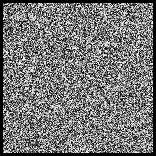
\includegraphics[width=3cm]{contents/chapter-2/2-contohcdp.jpg}
	\caption{Salah satu contoh CDP}
	\label{Fig: 2-contohcdp}
\end{figure}

CDP telah dicoba untuk dicetak menggunakan berbagai variasi \emph{printers}: \emph{Printer} kantor seperti \emph{inkjet} dan \emph{laser}, \emph{printer
	offset} dan \emph{digital offset}, dan juga \emph{printer} termal. Hasil percobaan dari pencetakan menggunakan beberapa jenis \emph{printer} tadi, semua CDP
salinan dapat dibedakan dengan CDP orisinal dengan margin yang cukup nyaman \cite{picard2004digital}, \cite{picard2004towards}, \cite{harwood1998optical}.

CDP sebaiknya tidak dianggap sebagai pesaing untuk perangkat keamanan optik lainnya, namun dijadikan sebagai alternatif yang lebih murah pada kasus-kasus
tertentu. Dengan memanfaatkan konsep degradasi gambar dan informasi yang tidak terancam oleh perkembangan perangkat pemindai dan pencetak digital, CDP menjadi
alternatif yang paling murah dalam memroteksi dokumen \cite{picard2004digital}, \cite{picard2004towards}, \cite{harwood1998optical}.

\subsection{Lokalisasi Objek dengan Pengenalan Pola}
Lokalisasi objek adalah proses mengidentifikasi posisi dan orientasi objek atau pola tertentu pada sebuah gambar menggunakan teknik pengolahan citra dan visi
komputer. Proses ini melibatkan deteksi objek atau pola dalam gambar serta mengestimasi lokasi dan orientasi yang tepat relatif terhadap kamera
\cite{sivic2003video}, \cite{liu2016ssd}.

Berbagai teknik telah diusulkan untuk melakukan lokalisasi objek atau gambar dengan pengenalan pola, termasuk deteksi fitur, pencocokan \emph{template}, dan
metode berbasis pembelajaran mesin. Teknik-teknik ini telah digunakan dalam berbagai aplikasi, seperti \emph{augmented reality}, robotika, dan pelacakan objek.

\subsection{ArUco \emph{Marker}}
ArUco \emph{marker} adalah jenis \emph{marker} fidusial yang biasa digunakan untuk estimasi pose kamera dan pelacakan dalam pengolahan citra dan visi komputer. ArUco \emph{marker} terdiri dari kisi-kisi kotak hitam dan putih dengan pola unik yang mudah dideteksi dan dikenali oleh algoritma visi komputer. ArUco \emph{marker} banyak digunakan dalam aplikasi robotika, realitas tambahan, dan pelacakan objek karena kesimpelannya, akurasi deteksi yang tinggi, dan biaya komputasi yang rendah \cite{arucoopencv}.

\emph{Marker} fidusial adalah objek berpola yang digunakan ke dalam sebuah gambar atau tempat tertentu untuk memudahkan sistem visi komputer menentukan posisi dan orientasi objek atau \emph{scene} dengan akurasi yang tinggi. \emph{Marker} fidusial biasanya didesain dengan pola atau bentuk yang unik dan mudah dikenali, sehingga dapat dideteksi dan dilacak oleh algoritme pendeteksian objek visi komputer, yang memungkinkan estimase pose dan pelacakan yang akurat. \emph{Marker} fidusial banyak digunakan dalam berbagai aplikasi seperti \emph{augmented reality}, robotika, dan pendeteksian objek \cite{arucoopencv}.

% \subsection{Ekstraksi Fitur pada Gambar}
\subsection{Fitur Spasial pada Citra Gambar}
Fitur spasial pada citra gambar adalah fitur yang berkaitan dengan letak, bentuk, dan struktur dari objek dalam citra. Fitur ini melibatkan ekstraksi informasi
spasial dari citra, seperti tingkat kecerahan, kejelasan, sudut, tepi, dan tekstur \cite{Gonzalez2009}.

Jenis fitur spasial yang umum digunakan dalam pemrosesan citra antara lain adalah \cite{Gonzalez2009}:

\begin{enumerate}
	\item Tepi: fitur yang mengidentifikasi perubahan tajam dalam intensitas piksel dalam citra dan digunakan untuk menghasilkan kontur atau garis tepi dari objek dalam
	      citra.
	\item Tekstur: fitur yang menggambarkan pola dan struktur permukaan dari objek dalam citra, seperti kekasaran, kepadatan, dan konsistensi.
	\item Ruang warna: fitur yang menggambarkan kualitas warna dan perbedaan warna dalam citra, seperti hue, saturasi, dan nilai.
	\item Bentuk: fitur yang mengidentifikasi bentuk dan ukuran objek dalam citra, seperti lingkaran, segitiga, atau persegi panjang.
\end{enumerate}

Fitur spasial ini dapat diekstraksi dan digunakan untuk melatih model deep learning untuk melakukan tugas tertentu pada citra, seperti klasifikasi objek,
deteksi objek, atau segmentasi citra. Dalam pemrosesan citra, fitur spasial merupakan komponen penting dalam analisis dan pengolahan citra \cite{Gonzalez2009}.

\subsection{Fitur Histogram pada Citra Gambar}
Histogram citra adalah grafik yang menunjukkan frekuensi kemunculan intensitas piksel dalam citra. Histogram digunakan untuk mengidentifikasi dan memahami
distribusi intensitas cahaya pada gambar. Histogram dapat digunakan dalam banyak aplikasi pemrosesan citra, seperti koreksi warna, segmentasi, ekstraksi fitur,
dan pengenalan pola \cite{fiturhistogram}. Gambar berwarna akan memiliki tiga histogram, satu untuk setiap saluran warna (merah, hijau, dan biru), sedangkan
gambar hitam-putih hanya akan memiliki satu histogram.

\begin{figure}[!ht]
	\centering
	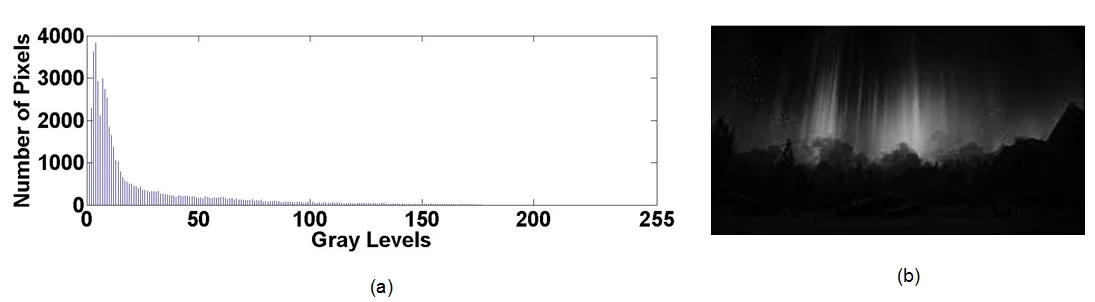
\includegraphics[width=7cm]{contents/chapter-2/2-histogramgelap.png}
	\caption[Histogram pada gambar dengan pencahayaan gelap]{Histogram pada gambar dengan pencahayaan gelap \cite{fiturhistogram}}
	\label{Fig: 2-histogramgelap}
\end{figure}

\begin{figure}[!ht]
	\centering
	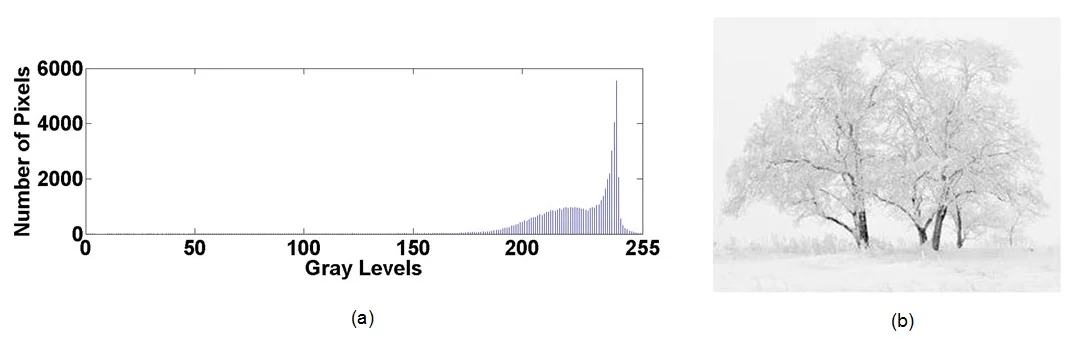
\includegraphics[width=7cm]{contents/chapter-2/2-histogramterang.png}
	\caption[Histogram pada gambar dengan pencahayaan terang]{Histogram pada gambar dengan pencahayaan terang \cite{fiturhistogram}}
	\label{Fig: 2-histogramterang}
\end{figure}

Histogram citra memiliki beberapa karakteristik penting yang dapat digunakan untuk analisis citra. Pertama, histogram dapat digunakan untuk melihat distribusi
level dari piksel gambar. Kedua, histogram dapat digunakan untuk mengidentifikasi kecerahan pada gambar, jika nilainya terkonsentrasi ke kiri, maka citra
gambar tersebut relatif gelap. Jika konsentrasinya condong ke kanan, maka citra gambar tersebut terang. Perbandingan distribusi histogram pada citra gambar
gelap dan terang dapat dilihat pada Gambar \ref{Fig: 2-histogramgelap} dan Gambar \ref{Fig: 2-histogramterang}.

\noindent Ketiga, histogram dapat digunakan untuk mengidentifikasi kontras pada citra gambar. Histogram yang terdistribusi secara merata menunjukkan bahwa gambar memiliki kontras yang baik, sedangkan histogram yang terdistribusi terfokus pada bagian tertentu menunjukkan kontras gambar yang rendah. Perbandingan distribusi histogram pada citra gambar kontras tinggi dan kontras rendah dapat dilihat pada Gambar \ref{Fig: 2-histogramkontrastinggi} dan Gambar \ref{Fig: 2-histogramkontrasrendah}.

\begin{figure}[!ht]
	\centering
	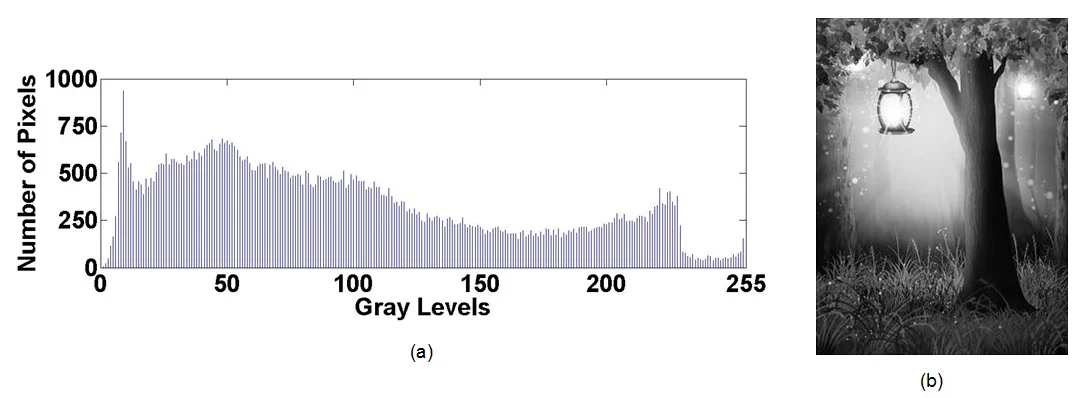
\includegraphics[width=10cm]{contents/chapter-2/2-histogramcontras.png}
	\caption[Histogram pada gambar dengan kontras tinggi]{Histogram pada gambar dengan kontras tinggi \cite{fiturhistogram}}
	\label{Fig: 2-histogramkontrastinggi}
\end{figure}

\begin{figure}[!ht]
	\centering
	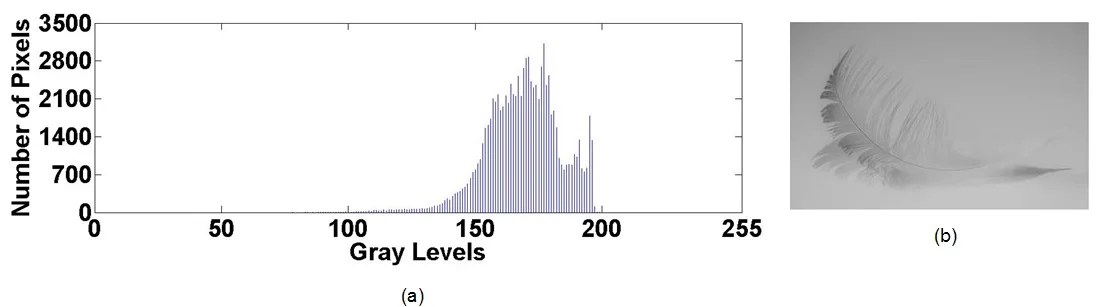
\includegraphics[width=10cm]{contents/chapter-2/2-histogramnoncontras.png}
	\caption[Histogram pada gambar dengan kontras rendah]{Histogram pada gambar dengan kontras rendah \cite{fiturhistogram}}
	\label{Fig: 2-histogramkontrasrendah}
\end{figure}

\noindent Keempat, histogram juga dapat digunakan untuk melihat efek saturasi pada gambar. Jika pada histogram terdapat nilai dengan \emph{spike} yang tinggi, hal tersebut berarti ada piksel gambar yang mengalami kerusakan akibat saturasi tinggi. Contoh distribusi histogram gambar yang memiliki saturasi tinggi dapat dilihat pada Gambar \ref{Fig: 2-histogramsaturasitinggi}

\begin{figure}[!ht]
	\centering
	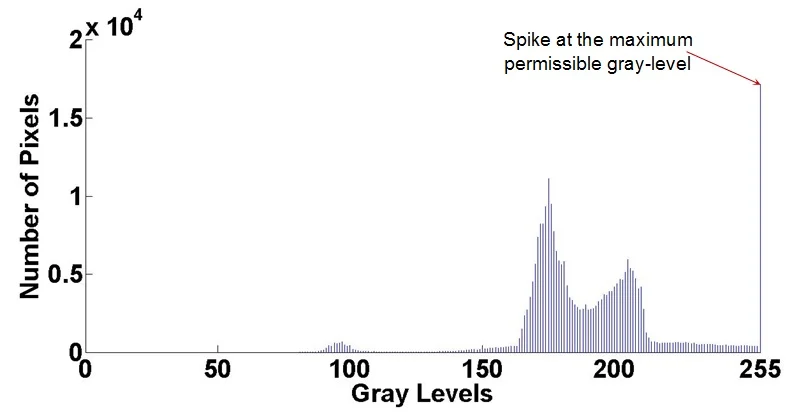
\includegraphics[width=7cm]{contents/chapter-2/2-histogramsaturasi.png}
	\caption[Histogram pada gambar dengan saturasi tinggi]{Histogram pada gambar dengan saturasi tinggi \cite{fiturhistogram}}
	\label{Fig: 2-histogramsaturasitinggi}
\end{figure}

\noindent Namun, fitur histogram dari sebuah citra gambar memiliki kelemahan, yaitu tidak memberikan informasi mengenai distribusi spasial dari nilai piksel citra gambar. Dengan demikian, dapat ditemui gambar berbeda yang memiliki distribusi histogram yang sama, seperti yang dapat dilihat pada Gambar \ref{Fig: 2-histogramdrawback}.

\begin{figure}[!ht]
	\centering
	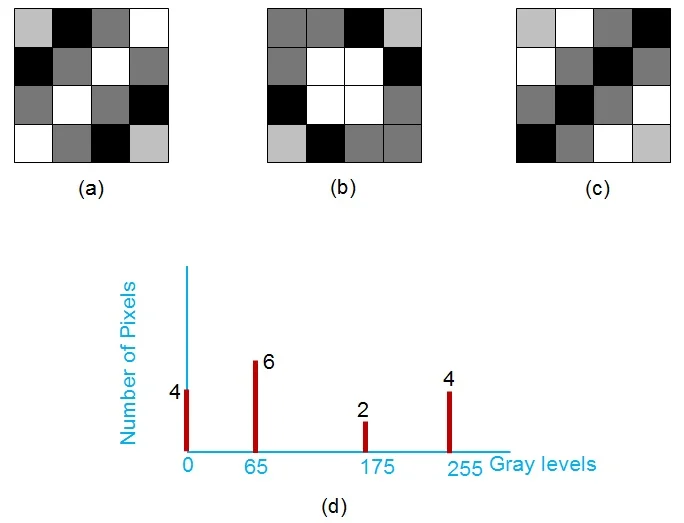
\includegraphics[width=6cm]{contents/chapter-2/2-histogramdrawback.png}
	\caption[Gambar yang berbeda memiliki distribusi histogram yang sama]{Gambar yang berbeda memiliki distribusi histogram yang sama \cite{fiturhistogram}}
	\label{Fig: 2-histogramdrawback}
\end{figure}

Fitur histogram pada gambar juga dapat digunakan untuk melakukan \emph{thresholding}, yaitu mengubah citra \emph{grayscale} yang bergradasi menjadi beberapa
level saja dengan ambang batas tertentu untuk tiap-tiap levelnya. Histogram merupakan salah satu cara mudah untuk mengidentifikasi ambang batas yang sesuai.
pada Gambar \ref{Fig: 2-histogramideal}, nilai piksel terkonsentrasi dalam dua kelompok, sehingga ambang batas dapat ditentukan yaitu nilai tengah kedua
kelompok tersebut. Pada Gambar \ref{Fig: 2-histogramnonideal}, sifat histogram lebih kontinyu, menunjukkan bahwa gambar tersebut bukan kandidat yang baik untuk
\emph{thresholding} karena untuk menentukan nilai pembatas yang ideal akan sulit.

\begin{figure}[!ht]
	\centering
	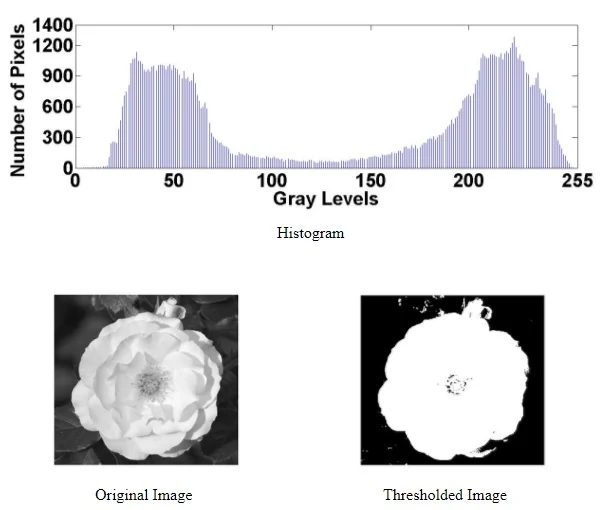
\includegraphics[width=6cm]{contents/chapter-2/2-histogramideal.png}
	\caption[Gambar yang ideal untuk di-\emph{thresholding}]{Gambar yang ideal untuk di-\emph{thresholding} \cite{fiturhistogram}}
	\label{Fig: 2-histogramideal}
\end{figure}

\begin{figure}[!ht]
	\centering
	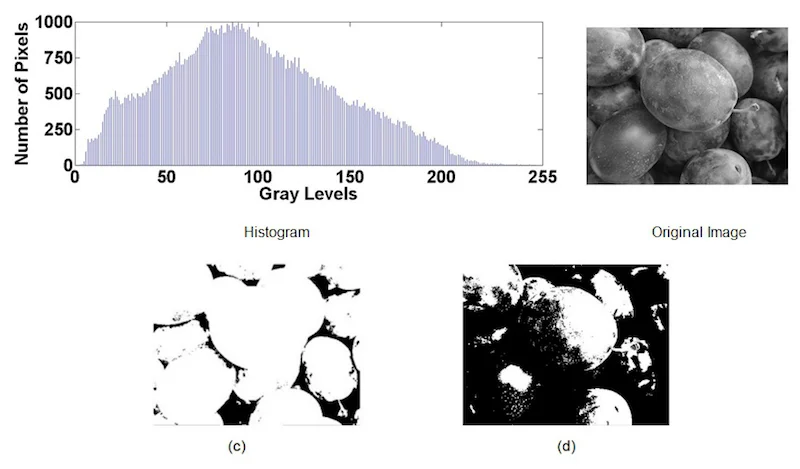
\includegraphics[width=6cm]{contents/chapter-2/2-histogramnonideal.png}
	\caption[Gambar yang tidak ideal untuk di-\emph{thresholding}]{Gambar yang tidak ideal untuk di-\emph{thresholding} \cite{fiturhistogram}}
	\label{Fig: 2-histogramnonideal}
\end{figure}

\clearpage

\subsection{Fitur DCT pada Citra Gambar}
DCT (\emph{Discrete Cosine Transform}) adalah transformasi matematis yang digunakan untuk mengubah sinyal digital atau data spasial menjadi domain frekuensi.
DCT menghasilkan serangkaian koefisien frekuensi yang merepresentasikan sinyal atau data spasial dalam bentuk domain frekuensi. Dalam domain frekuensi, sinyal
atau data citra direpresentasikan oleh koefisien-koefisien frekuensi. DCT memanfaatkan sifat alami dari citra dan memungkinkan informasi citra yang relevan
dikonsentrasikan dalam beberapa koefisien frekuensi teratas, sedangkan koefisien frekuensi yang lain diabaikan atau dikuantisasi dengan rinci. Transformasi ini
banyak digunakan dalam pengolahan sinyal, pengolahan citra, dan kompresi data, seperti pada format file JPEG dan MP3 \cite{dct}.

Dalam aplikasi pengolahan citra, DCT digunakan untuk menghasilkan representasi domain frekuensi dari citra digital. Hal ini memungkinkan penghapusan informasi
yang tidak penting pada citra. Dalam kompresi audio, DCT digunakan untuk memisahkan sinyal audio menjadi beberapa subband frekuensi \cite{dct}.

DCT juga banyak digunakan pada pembandingan citra dan gambar. Teknik ini dapat digunakan untuk mendeteksi keaslian citra dan \emph{watermarking}. Dalam
pembandingan citra dan gambar, DCT digunakan untuk memperoleh fitur-fitur citra yang berbeda. Fitur-fitur ini kemudian digunakan untuk menghitung kesamaan
antara dua citra atau gambar. Dalam aplikasi deteksi keaslian citra, DCT dapat digunakan untuk menghasilkan \emph{signature} unik dari setiap citra asli.
Sementara dalam \emph{watermarking}, DCT digunakan untuk memasukkan \emph{watermark} atau pesan rahasia ke dalam citra \cite{dctwatermark}.

Secara umum, persamaan DCT pada citra 2 dimensi (gambar berukuran N x M) didefinisikan dengan \cite{dct}:

\begin{equation}
	\resizebox{.9\hsize}{!}{$F(u,v) = \left(\frac{2}{N}\right)^{\frac{1}{2}}\left(\frac{2}{M}\right)^{\frac{1}{2}}\sum_{i=0}^{N-1}\sum_{j=0}^{M-1}\Lambda(i).\Lambda(j).cos\left[\frac{\pi.u}{2.N}(2i+1)\right]cos\left[\frac{\pi.v}{2.M}(2j+1) \right].f(i,j)$}
\end{equation}

\subsection{Koefisien Jarak}
Koefisien jarak merupakan ukuran atau besaran yang menggambarkan seberapa dekat atau jauh dua objek dalam ruang atau dimensi tertentu. Koefisien jarak dapat
digunakan untuk mengukur kesamaan atau perbedaan antara dua objek yang diamati. Ada beberapa koefisien jarak yang sering digunakan, antara lain:

\subsubsection{Koefisien Jarak Euclidean}
Jarak \emph{euclidean} adalah ukuran jarak yang paling umum digunakan dalam matematika dan ilmu komputer untuk mengukur jarak antara dua titik dalam ruang \emph{euclidean}
n-dimensi. Jarak \emph{euclidean} dihitung sebagai akar kuadrat dari jumlah kuadrat perbedaan koordinat antara dua titik. Secara formal, jarak \emph{euclidean} antara dua
vektor $u$ dan $v$ dalam ruang \emph{euclidean} n-dimensi didefinisikan sebagai:

\begin{equation}
	d(u,v) = \sqrt{\sum_{i=1}^{n}(u_i - v_i)^2}
\end{equation}

\noindent di mana $n$ adalah jumlah dimensi dalam \emph{vector space}, dan $u_i$ dan $v_i$ merepresentasikan komponen ke-$i$ pada vektor.

\subsubsection{Koefisien Jarak Korelasi}
Koefisien jarak korelasi adalah suatu ukuran kemiripan atau perbedaan antara dua vektor, berdasarkan korelasi antara komponen-komponennya. Nilai dari jarak
korelasi dinormalisasi antara 0 dan 1, di mana 0 menunjukkan korelasi positif sempurna sedangkan 1 menunjukkan korelasi negatif sempurna.

Untuk menghitung jarak korelasi antara dua vektor $u$ dan $v$, dapat dituliskan dengan:

\begin{equation}
	d(u,v) = 1-\frac{(u-\bar{u})\cdot (v-\bar{v})}{\Vert(u-\bar{u})\Vert_2\Vert(v-\bar{v})\Vert_2}
\end{equation}

\noindent di mana $d(u, v)$ adalah jarak korelasi antara $u$ dan $v$, $\bar{v}$ adalah rata-rata elemen dari vektor $v$, dan $x\cdot y$ adalah \emph{dot product} dari $x$ dan $y$. Jarak korelasi sering digunakan dalam algoritma pengelompokan dan klasifikasi untuk mengukur perbedaan antara sampel, terutama ketika vektor memiliki banyak komponen dan data sangat berkorelasi.

\subsubsection{Koefisien Jarak Kosinus}
Koefisien jarak kosinus adalah sebuah metode untuk mengukur kemiripan antara dua vektor dalam ruang n-dimensi \cite{schutze2008introduction},
\cite{deisenroth2020mathematics}. Metode ini mengukur sudut antara dua vektor dan menghasilkan nilai berkisar antara 0 dan 1, di mana 0 menunjukkan bahwa
vektor tersebut saling tegak lurus, sedangkan 1 menunjukkan bahwa vektoor tersebut saling sejajar. Semakin kecil nilai koefisien jarak kosinus, semakin mirip
kedua vektor tersebut. Jarak kosinus antara dua vektor $u$ dan $v$ dapat dituliskan sebagai berikut:

\begin{equation}
	d(u,v) = 1-\frac{u\cdot v}{\Vert u\Vert_2\Vert v\Vert_2}
\end{equation}

\noindent di mana $u\cdot v$ adalah hasil \emph{dot product} antara vektor $u$ dan $v$, sedangkan $\Vert u\Vert_2$ dan $\Vert v\Vert_2$ adalah panjang dari vektor $u$ dan $v$.

\subsubsection{Koefisien Jarak Canberra}
Jarak Canberra adalah salah satu metode mengukur jarak antara dua vektor dalam ruang n-dimensi. Metode ini mengevaluasi perbedaan proporsional antara
nilai-nilai pada setiap elemen vektor. Metode ini sering digunakan dalam analisis data untuk mengukur kemiripan antara dua set data numerik
\cite{clusteringSumayiaAlAnazi}, \cite{sneath1973numerical}. Secara formal, perhitungan jarak canberra antara dua vektor $u$ dan $v$ adalah:

\begin{equation}
	d(u,v) = \sum_i\frac{\left | u_i-v_i \right |}{\left | u_i \right |+\left | v_i \right |}
\end{equation}

\subsection{Transformasi Homografi}
Transformasi homografi adalah sebuah transformasi geometri pada ruang n-dimensi yang memetakan setiap titik pada bidang ke titik yang sesuai pada bidang
lainnya, dengan menerapkan konsep persamaan linier homogen. Transformasi homografi dapat mengubah ukuran, rotasi, dan persepektif dari gambar atau objek pada
bidang ruang n-dimensi.

Transformasi homografi biasanya dilakukan dalam ruang koordinat \emph{homogeneous}, yang merupakan ruang n+1 dimensi dengan koordinat homogen yang memungkinkan
dilakukannya transformasi perspektif. Dalam ruang koordinat \emph{homogeneous}, sebuah titik pada bidang n-dimensi dinyatakan dalam bentuk vektor homogen (x,
y, z, w), di mana x, y, dan z adalah koordinat euclidean, dan w adalah koordinat homogen. 
% Sebuah matriks homografi H juga dinyatakan dalam bentuk matriks
% homogen:

% \begin{equation}
% 	\begin{bmatrix}
% 		x' \\
% 		y' \\
% 		w'
% 	\end{bmatrix}=H\begin{bmatrix}
% 		x \\
% 		y \\
% 		w
% 	\end{bmatrix}
% \end{equation}

\subsection{Uji Statistik \emph{T-test}}
Uji statistik \emph{T-test} adalah sebuah teknik statistik yang digunakan untuk membandingkan rata-rata dari dua sampel independen. Uji ini menghasilkan nilai \emph{t-statistics} dan \emph{p-value} yang dapat digunakan untuk menentukan apakah perbedaan antara kedua sampel signifikan secara statistik \cite{kumar}.

\emph{T-statistics} adalah ukuran dari perbedaan rata-rata antara dua sampel, yang dinormalisasi dengan standar deviasi dari kedua sampel. Semakin besar nilai \emph{t-statistics}, semakin signifikan perbedaan antara kedua sampel. \emph{P-value} adalah nilai probabilitas yang diperoleh dari perhitungan statistik, dan menunjukkan seberapa signifikan perbedaan tersebut. Semakin kecil nilai \emph{P-value}, semakin signifikan perbedaan antara kedua sampel \cite{kumar}.

Dalam uji statistik \emph{T-test} untuk dua sampel independen, hipotesis nol menyatakan bahwa tidak ada perbedaan yang signifikan antara kedua sampel. Jika
\emph{P-value} kurang dari alfa (tingkat signifikansi yang telah ditentukan sebelumnya), maka hipotesis nol ditolak dan dapat disimpulkan bahwa terdapat
perbedaan signifikan antara kedua sampel \cite{kumar}. 

\noindent Definisi formal dari uji statistik \emph{T-test} dapat dituliskan dengan \cite{kumar}:

\begin{equation}
	t = \frac{\bar{x}_1 - \bar{x}_2}{\sqrt{\frac{s_1^2}{n_1} + \frac{s_2^2}{n_2}}}
\end{equation}

di mana $\bar{x}_1$ and $\bar{x}_2$ adalah rata-rata dari sampel, $s_1$ dan $s_2$ adalah standar deviasi sampel, dan $n_1$ dan $n_2$ adalah ukuran sampel.

\subsection{Pembelajaran Mesin}
Pembelajaran mesin adalah sebuah cabang dari kecerdasan buatan yang memungkinkan sistem komputer untuk belajar dari data, mengidentifikasi pola, dan melakukan
prediksi dalam menyelesaikan permasalahan. Secara umum, pembelajaran mesin mencoba untuk menemukan pola tersembunyi dalam data dan mempergunakan informasi
tersebut untuk menghasilkan hasil yang lebih baik dalam setiap iterasinya.

Sistem pembelajaran mesin dilatih dengan menggunakan data masukan dan berbagai teknik pemrosesan data untuk menghasilkan output yang diharapkan. Proses
pembelajaran ini melibatkan pembuatan model matematis dan analisis data. Dalam pembelajaran mesin, data digunakan untuk melatih model atau algoritma, sehingga
sistem dapat belajar dan meningkatkan kinerjanya dalam memecahkan masalah atau menyelesaikan tugas tertentu. Secara umum, ada tiga jenis pembelajaran mesin,
yaitu \emph{supervised learning}, \emph{unsupervised learning}, dan \emph{reinforcement learning}. \emph{Supervised learning} melibatkan penggunaan data yang
telah dilabeli atau dikategorikan sebelumnya untuk melatih model atau algoritma. \emph{Unsupervised learning} melibatkan penggunaan data yang belum dilabeli
atau dikategorikan sebelumnya untuk menemukan pola atau struktur yang terdapat dalam data. Sedangkan \emph{reinforcement learning} melibatkan penggunaan sistem
\emph{reward} dan \emph{punishment} untuk melatih model atau algoritma.

Dalam praktiknya, pembelajaran mesin sering digunakan dalam berbagai aplikasi bisnis, seperti analisis data, personalisasi produk, dan deteksi kecurangan.
Dalam kehidupan sehari-hari, pembelajaran mesin juga diterapkan dalam pengenalan suara, identifikasi gambar, dan pengembangan sistem kendali otomatis \cite{jordan2015machine}, \cite{Alpaydin2014}, \cite{murphy2012machine}.

\subsection{AutoML}
AutoML (\emph{Automated Machine Learning}) adalah teknologi yang dirancang untuk memudahkan proses pembuatan model pembelajaran mesin secara otomatis. AutoML
semakin populer karena memungkinkan organisasi dan perusahaan untuk menghasilkan model pembelajaran mesin secara cepat dan efisien, sehingga mempercepat
inovasi dan pengambilan keputusan dalam bisnis. Namun, AutoML bukanlah solusi yang sempurna dan masih memiliki beberapa tantangan seperti kurangnya
interpretasi model dan pengurangan fleksibilitas dalam menghasilkan model yang dapat disesuaikan dengan kebutuhan khusus \cite{manashgoswami_2023},
\cite{singla_2020}.

AutoML memungkinkan otomatisasi dari beberapa tahapan dalam proses pengembangan model, seperti \emph{pre-processing}, \emph{feature selection},
\emph{hyperparameter tuning}, dan \emph{model selection}. Tujuan dari AutoML adalah untuk mengurangi waktu dan biaya dalam pengembangan model pembelajaran
mesin, dan memungkinkan pengguna yang tidak berpengalaman dalam machine learning untuk menghasilkan model yang dapat digunakan dalam berbagai aplikasi \cite{manashgoswami_2023}, \cite{singla_2020}.

AutoML dapat menangani berbagai jenis tugas, termasuk klasifikasi, regresi, klastering, dan segmentasi. Selain itu, AutoML juga dapat mengolah berbagai jenis
data, seperti data tabular, gambar, dan teks. Dalam pengolahan data tabular, AutoML dapat mengidentifikasi tipe data yang berbeda, seperti numerik dan
kategorikal, dan secara otomatis melakukan pra-pemrosesan data, seperti normalisasi, pengisian nilai yang hilang, dan pemilihan fitur. Sampai saat ini, AutoML
optimal digunakan pada data berjenis tabular \cite{manashgoswami_2023}, \cite{singla_2020}.

Adapun \emph{framework} AutoML populer yang dikembangkan, baik bersifat \emph{open} ataupun \emph{closed source}, seperti Auto-WEKA, auto-sklearn, GCP-Tables,
TPOT, H2O, AutoGluon, dan masih banyak lagi. \emph{Framework} AutoMl tersebut sudah banyak digunakan di industri dan terkadang memiliki akurasi yang jauh lebih
baik dibandingkan model yang dibuat secara manual \cite{agtabular}.

\subsection{AutoGluon} \label{AutoGluon}
AutoGluon merupakan \emph{framework} \emph{machine learning} (ML) dan \emph{deep learning} (DL) sumber terbuka yang memungkinkan pengguna untuk membuat model
ML ataupun DL yang akurat dan optimal dengan mudah. \emph{Framework} ini dikembangkan oleh AutoGluon Inc., dan dirilis pertama pada tahun 2019 dengan dukungan
penuh pada Python versi 3. Berbeda dengan model lain yang fokus pada pemilihan model dan \emph{hyperparameter}, AutoGluon sukses membuat model yang lebih baik
dengan teknik \emph{ensembling} beberapa model dan melakukan \emph{stacking} model-model tersebut pada \emph{multi-layer}. Dari hasil eksperimen oleh tim, pada
rangkaian 50 tes permsalahan klasifikasi dan regresi dari Kaggle, AutoGluon lebih cepat, kokoh, dan jauh lebih akurat dari beberapa model AutoML lain yang
terkenal seperti TPOT, H2O, AutoWEKA, auto-sklearn, dan Google AutoML Tables. Melalui kompetisi Kaggle, AutoGluon bahkan sering mengungguli kompetitornya yang
merupakan ekspert data \emph{scientist}. Bahkan, pada 2 kompetisi Kaggle populer, AutoGluon mengalahkan 99\% partisipan yang merupakan \emph{data scientist}
dan juga pengembang model AutoML lain \cite{agtabular}.

AutoGluon menyediakan antarmuka yang mudah digunakan, namun juga menyediakan fleksibilitas yang cukup bagi pengguna. Beberapa fitur utama dari AutoGluon adalah
sebagai berikut:

\begin{itemize}
	\item AutoML: Autogluon memiliki kemampuan untuk membuat model \emph{automated machine learning} yang memungkinkan pengguna untuk secara otomatis menyelesaikan tugas
	      seperti klasifikasi, regresi, dan deteksi objek. AutoGluon dapat bekerja pada data tabular, multimodal, maupun \emph{time-series}.
	\item Pemilihan model otomatis.
	\item Model \emph{ensembling}.
	\item Penyetelan \emph{hyperparameter}.
	\item Pemrosesan fitur (\emph{feature} engineering).
	\item Data \emph{preprocessing}.
	\item Pemisahan data (data \emph{splitting}).
\end{itemize}

AutoGluon memiliki performa yang sangat baik apabila dibandingkan AutoML kompetitor seperti H2O, TPOT, GCP-Tables, auto-sklearn, dan Auto-WEKA. Pada Tabel
\ref{Tab: 2-hasilautogluon}, terlihat bahwa AutoGluon jauh mengungguli kompetitornya. Dari pengujian menggunakan 39 \emph{dataset}, AutoGluon berhasil menjadi
juara dengan akurasi terbaik pada 23 \emph{dataset}. Rata-rata waktu \emph{training} AutoGluon juga sangat baik dibandingkan kompetitornya, hanya kalah dari
GCP-Tables \cite{agtabular}.

\begin{table}[!ht]
	\centering
	\caption[Perbandingan performa AutoGluon dengan AutoML kompetitor]{Perbandingan performa AutoGluon dengan AutoML kompetitor \cite{agtabular}}
	\vspace{0.5em}
	\resizebox{\textwidth}{!}{\begin{tabular}{|c|c|c|c|c|c|c|c|}
			\hline
			\textbf{Framework}    & \textbf{Wins} & \textbf{Losses} & \textbf{Failures} & \textbf{Champion} & \textbf{Avg. Rank} & \textbf{Avg. Rescaled Loss} & \textbf{Avg. Time (min)} \\ \hline
			\textbf{AutoGluon}    & -             & -               & \textbf{1}        & \textbf{23}       & \textbf{1.8438}    & \textbf{0.1385}             & 201                      \\ \hline
			\textbf{H2O AutoML}   & 4             & 26              & 8                 & 2                 & 3.125              & 0.2447                      & 220                      \\ \hline
			\textbf{TPOT}         & 6             & 27              & 5                 & 5                 & 3.375              & 0.2034                      & 235                      \\ \hline
			\textbf{GCP-Tables}   & 5             & 20              & 14                & 4                 & 3.75               & 0.3336                      & \textbf{195}             \\ \hline
			\textbf{auto-sklearn} & 6             & 27              & 6                 & 3                 & 3.8125             & 0.3197                      & 240                      \\ \hline
			\textbf{Auto-WEKA}    & 4             & 28              & 6                 & 1                 & 5.0938             & 0.8001                      & 244                      \\ \hline
		\end{tabular}}
	\label{Tab: 2-hasilautogluon}
\end{table}